\documentclass[12pt]{article}
\usepackage{amsthm,amssymb,amsfonts,amsmath,amstext,systeme,graphicx,float,tabularx}
\marginparwidth 0pt
\oddsidemargin -1.2 truecm
\evensidemargin  0pt 
\marginparsep 0pt
\topmargin -2.2truecm
\linespread{1}
\textheight 25.8 truecm
\textwidth 18.5 truecm
\newenvironment{remark}{\noindent{\bf Remark }}{\vspace{0mm}}
\newenvironment{remarks}{\noindent{\bf Remarks }}{\vspace{0mm}}
\newenvironment{question}{\noindent{\bf Question }}{\vspace{0mm}}
\newenvironment{questions}{\noindent{\bf Questions }}{\vspace{0mm}}
\newenvironment{note}{\noindent{\bf Note }}{\vspace{0mm}}
\newenvironment{summary}{\noindent{\bf Summary }}{\vspace{0mm}}
\newenvironment{back}{\noindent{\bf Background}}{\vspace{0mm}}
\newenvironment{conclude}{\noindent{\bf Conclusion}}{\vspace{0mm}}
\newenvironment{concludes}{\noindent{\bf Conclusions}}{\vspace{0mm}}
\newenvironment{dill}{\noindent{\bf Description of Dill's model}}{\vspace{0mm}}
\newenvironment{maths}{\noindent{\bf Mathematics needed}}{\vspace{0mm}}
\newenvironment{inst}{\noindent{\bf Instructions}}{\vspace{0mm}}
\newenvironment{notes}{\noindent{\bf Notes }}{\vspace{0mm}}
\newenvironment{theorem}{\noindent{\bf Theorem }}{\vspace{0mm}}
\newenvironment{example}{\noindent{\bf Example }}{\vspace{0mm}}
\newenvironment{examples}{\noindent{\bf Examples }}{\vspace{0mm}}
\newenvironment{topics}{\noindent{\bf Topics}}{\vspace{0mm}}
\newenvironment{outcomes}{\noindent{\bf Expected Learning Outcomes}}{\vspace{0mm}}
\newenvironment{lemma}{\noindent{\bf Lemma }}{\vspace{0mm}}
\newenvironment{solution}{\noindent{\it Solution}}{\vspace{2mm}}
\newcommand{\ds}{\displaystyle}
\newcommand{\un}{\underline}
\newcommand{\bs}{\boldsymbol}

\begin{document}

\baselineskip 18 pt
\begin{center}
	{\large \bf Function By Topic}
\end{center}
\vspace{0.05cm}

\begin{enumerate}
	\item \textbf{HKDSE MATH CORE 2012 Past Paper I Q13}
	\begin{enumerate}
		\item[(a)] Find the value of $k$ such that $x - 2$ is a factor of $kx^3 - 21x^2 + 24x - 4$. \\(2 marks)
		\item[(b)] Figure 4 shows the graph of $y = 15x^2 - 63x + 72$. $Q$ is a variable point on the graph in the first quadrant. $P$ and $R$ are the feet of the perpendiculars from $Q$ to the $x$-axis and the $y$-axis respectively.
		\begin{figure}[H]
			\centering
			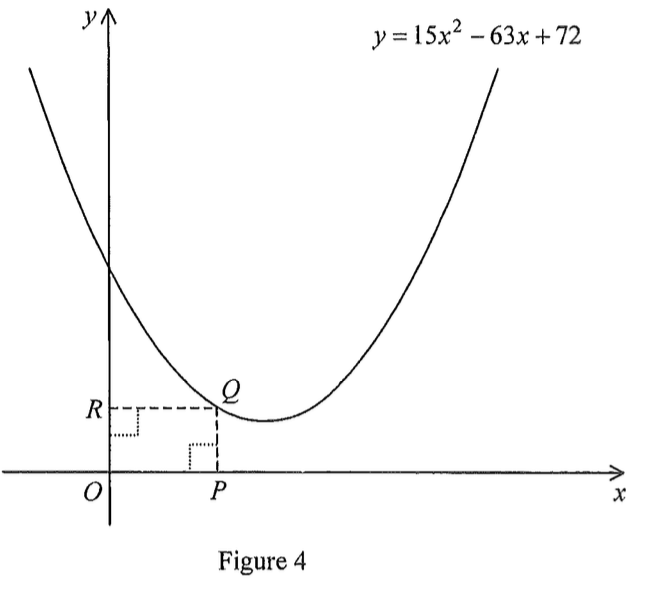
\includegraphics[width = .3\linewidth]{2012Figure1.4}
		\end{figure}
		\begin{enumerate}
			\item[(i)] Let $(m, 0)$ be the coordinates of $P$. Express the area of the rectangle $OPQR$ in terms of $m$.
			\item[(ii)] Are there three different positions of $Q$ such that the area of the rectangle $OPQR$ is 12? Explain your answer.
		\end{enumerate}
		(5 marks)
	\end{enumerate}
	
	\item \textbf{HKDSE MATH CORE 2013 Past Paper I Q12}\\
	Let  $f(x) = 3x^3 - 7x^2 + kx - 8$, where $k$ is a constant. It is given that $f(x) \equiv (x - 2)(ax^2 + bx + c)$, where $a$, $b$ and $c$ are constants.
	\begin{enumerate}
		\item[(a)] Find $a$, $b$ and $c$. \\(4 marks)
		\item[(b)] Someone claims that all the roots of the equation  $f(x) = 0$ are real numbers. Do you agree? Explain your answer. \\(3 marks)
	\end{enumerate}

	\item \textbf{HKDSE MATH CORE 2014 Past Paper I Q13}\\
	It is given that $f(x)$ is the sum of two parts, one part varies as $x^2$ and the other part is a constant. Suppose that $f(2) = 59$ and $f(7) = -121$.
	\begin{enumerate}
		\item[(a)] Find $f(6)$. \\(4 marks)
		\item[(b)] $A(6, a)$ and $B(-6, b)$ are points lying on the graph of $y = f(x)$. Find the area of $\triangle ABC$, where $C$ is a point lying on the $x$-axis. \\(4 marks)
	\end{enumerate}

	\newpage

	\item \textbf{HKDSE MATH CORE 2015 Past Paper I Q11}\\
	Let $f(x) = (x - 2)^2(x+h)+k$, where $h$ and $k$ are constants. When  $f(x)$ is divided by $x - 2$, the remainder is 5. It is given that  $f(x)$ is divisible by $x - 3$.
	\begin{enumerate}
		\item[(a)] Find $h$ and $k$. \\(3 marks)
		\item[(b)] Someone claims that all the roots of the equation  $f(x) = 0$ are integers. Do you agree? Explain your answer. \\(3 marks)
	\end{enumerate}

	\item \textbf{HKDSE MATH CORE 2016 Past Paper I Q14}\\
	Let $p(x) = 6x^4 + 7x^3 + ax^2 + bx + c$, where $a$, $b$ and $c$ are constants. When $p(x)$ is divided by $x + 2$ and when $p(x)$ is divided by $x - 2$, the two remainders are equal. It is given that $p(x) \equiv (lx^2 + 5x + 8)(2x^2 + mx + n)$, where $l$, $m$ and $n$ are constants.
	\begin{enumerate}
		\item[(a)] Find $l$, $m$ and $n$. \\(5 marks)
		\item[(b)] How many real roots does the equation $p(x) = 0$ have? Explain your answer. \\(5 marks)
	\end{enumerate}

	\item \textbf{HKDSE MATH CORE 2017 Past Paper I Q14}\\
	Let $f(x) = 6x^3 - 13x^2 - 46x + 34$. When $f(x)$ is divided by $2x^2 + ax + 4$, the quotient and the remainder are $3x + 7$ and $bx + c$ respectively, where $a$, $b$ and $c$ are constants.
	\begin{enumerate}
		\item[(a)] Find $a$. \\(3 marks)
		\item[(b)] Let $g(x)$ be a quadratic polynomial such that when $g(x)$ is divided by $2x^2 + ax + 4$, the remainder is $bx + c$.
		\begin{enumerate}
			\item[(i)] Prove that  $f(x) - g(x)$ is divisible by $2x^2 + ax + 4$.
			\item[(ii)] Someone claims that all the roots of the equation  $f(x) - g(x) = 0$ are integers. Do you agree? Explain your answer.
		\end{enumerate}
		(5 marks)
	\end{enumerate}

	\item \textbf{HKDSE MATH CORE 2018 Past Paper I Q12}\\
	Let $f(x) = 4x(x+1)^2 + ax + b$, where $a$ and $b$ are constants. It is given that $x - 3$ is a factor of $f(x)$. When $f(x)$ is divided by $x + 2$, the remainder is $2b + 165$.
	\begin{enumerate}
		\item[(a)] Find $a$ and $b$. \\(3 marks)
		\item[(b)] Someone claims that the equation $f(x) = 0$ has at least one irrational root. Do you agree? Explain your answer. \\(4 marks)
	\end{enumerate}

	\item \textbf{HKDSE MATH CORE 2019 Past Paper I Q11}\\
	Let $p(X)$ be a cubic polynomial. When $p(x)$ is divided by $x - 1$, the remainder is 50. When $p(X)$ is divided by $x + 2$, the remainder is $-52$. It is given that $p(x)$ is divisible by $2x^2 + 9x + 14$.
	\begin{enumerate}
		\item[(a)] Find the quotient when $p(X)$ is divided by $2x^2 + 9x + 14$. \\(3 marks)
		\item[(b)] How many rational roots does the equation   have? Explain your answer. \\(3 marks)
	\end{enumerate}

	\item \textbf{HKDSE MATH CORE 2020 Past Paper I Q13}\\
	The cubic polynomial $f(x)$ is divisible by $x-1$. When $f(x)$ is divided by $x^2-1$, the remainder is $kx+8$, where $k$ is a constant.
	\begin{enumerate}
		\item[(a)] Find $k$. \\(3 marks)
		\item[(b)] It is given that $x+3$ is a factor of $f(x)$. When $f(x)$ is divided by $x$, the remainder is 24. Someone claims that all the roots of the equation $f(x) = 0$ are integers. Is the claim correct? Explain your answer. \\(5 marks)
	\end{enumerate}

	\item \textbf{HKDSE MATH CORE 2021 Past Paper I Q12}\\	
	The polynomial $p(x)$ is divisible by $x - 5$. When $p(x)$ is divided by $x^2 + x + 1$, the quotient and the remainder are $2x^2 - 37$ and $cx + c - 1$ respectively, where $c$ is a constant.
	\begin{enumerate}
		\item[(a)] Find $c$. \\(3 marks)
		\item[(b)] Prove that $x+3$ is a factor of $p(x)$. \\(1 marks)
		\item[(c)] Someone claims that all the roots of the equation $p(x) = 0$ are real numbers. Is the claim correct? Explain your answer. \\(3 marks)
	\end{enumerate}

	\item \textbf{HKDSE MATH CORE 2022 Past Paper I Q14}\\
	Let $p(x) = 2x^3 + ax^2 + bx - 20$, where $a$ and $b$ are constants. When $p(x)$ is divided by $x^2 - 2x + 3$, the remainder is $x + 13$.
	\begin{enumerate}
		\item[(a)] Find $a$ and $b$. \\(3 marks)
		\item[(b)] Is $x - 5$ a factor of $p(x)$? Explain your answer. \\(2 marks)
		\item[(c)] Someone claims that the equation $p(x) = 0$ has two irrational roots. Do you agree? Explain your answer. \\(3 marks)
	\end{enumerate}


	\item \textbf{HKDSE MATH CORE 2023 Past Paper I Q13}\\
	Define $g(x) = x^3 + 5x^2 - 12x - 1$. Let $h(x) = 3x^4 + ax^3 - 16x^2 + bx + c$, where $a$, $b$ and $c$ are constants. When $h(x)$ is divided by $g(x)$, the quotient and the remainder are equal.
	\begin{enumerate}
		\item[(a)] Find the quotient when $h(x)$ is divided by $g(x)$. \\(3 marks)
		\item[(b)] How many rational roots does the equation $h(x) = 0$ have? Explain your answer. \\(4 marks)
	\end{enumerate}




\end{enumerate}








\end{document}